\documentclass[12pt,fleqn]{article}\usepackage{../../common}
\begin{document}
Kısıtlı Boltzmann Makinaları (Restricted Boltzmann Machines -RBM-)

RBM aynen Boltzman Makinalarında (BM) örneğinde olduğu gibi bir
dağılımdır. Verilen $x,h$ için bir olasılık değeri geri döndürebilir.
$$ p(x,h;W) = \exp (-E(x,h)) / Z $$

Standart RBM için $h,x$ ikiseldir (binary). Gizli (hidden) tabaka $h$, ve
``görünen (visible)'' tabaka $x$ vardır. $Z$ aynen önce gördüğümüz BM'de
olduğu gibi normalizasyon sabitidir. Spesifik bir RBM'i tanımlayan şey onun
$W$ matrisidir. Gizli değişkenler bazen karışıklık yaratabiliyor, bu
değişkenler aynen görünen değişkenler gibi değişkendirler. Yani belli
$h$'lerin ``olasılığı'' sorulabilir, ya da onlar üretilebilir. Fakat RBM'i
eğitirken sadece görünen kısmı tarafından eğitiriz. Gizli tabaka bu sırada
örneklem ile arada sırada içi doldurulur, bu tabii ki $W$'ye bağlı olarak
yapılacaktır. Gizli tabaka daha düşük boyutlu olduğu, ve 0/1 değerlerine
sahip olması mecbur olduğu için bu git/gel bir tür özetleme yapar ki
öğrenim bu sırada ortaya çıkar.

Devam edelim, $E$ tanımına ``enerji'' olarak ta atıf yapılabiliyor.

$$ E(x,h) = -h^TWx - c^Tx - b^Th $$

BM'lerden farklı olarak RBM'de $c,b$ değişkenleri var. Bu değişkenler
yanlılık (bias) için, yani veri içindeki genel eğilimi saptamaları için
modele konulmuştur. Ayrıca $h^TWx$ terimi var, bu BM'deki $x^TWx$'den biraz
farklı, daha önce belirttiğimiz gibi, $h$ üzerinden $x$'ler arasında
bağlantı yapıyor. BM ile tüm $x$ öğeleri birbirine bağlanabiliyordu, RBM
ile $h$ katmanında bağlantılar paylaşılıyor. Bu $h$ üzerinden bağlantı
zorunluluğu RBM'in özetleme alanını azaltarak genelleme oluşturmasını
sağlıyor. Bu yüzden onlara ``kısıtlı'' Boltzmann makinaları adı
veriliyor. Gizli değişkenlerin kendi aralarında, ve görünen değişkenlerin
kendi aralarında direk bağlantıya izin verilmemiştir, ki bu daha önce
bahsedilen kısıtlamanın bir diğer yönü. Bağlantılara, $W$ üzerinden sadece
gizli ve görünen değişkenler (tabakalar) arasında izin verilmiştir. Bu
ayrıca matematiksel olarak bazı kolaylıklar sağlıyor, bu konuyu birazdan
işleyeceğiz.

Formül alttaki gibi de açılabilir,

$$ = - \sum_j \sum_k W_{j,k}h_jx_k - \sum_k c_kx_k - \sum_j b_jh_j  $$

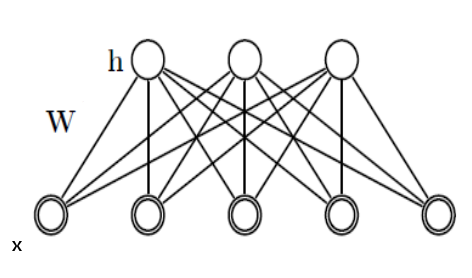
\includegraphics[height=4cm]{rbm_01.png}
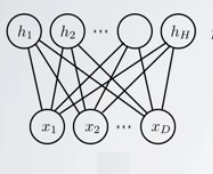
\includegraphics[height=4cm]{rbm_02.png}

Tekrar vurgulayalım, $h,x$ değişkenleri olasılık teorisinden bilinen
rasgele değişkenlerdir, yani hem $x$'e hem de $h$'e ``zar attırabiliriz'' /
bu değişkenler üzerinden örneklem toplayabiliriz.

Ayrıca, RBM'ler aynen BM'ler gibi bir olasılık yoğunluk fonksiyonu
üzerinden tanımlanırlar, önceki formülde gördüğümüz gibi, tüm mümkün
değerleri üzerinden entegralleri (ya da toplamları) alınınca sonuç 1 olur,
vs.

Devam edelim, ana formülden hareketle cebirsel olarak şunlar da doğrudur,

$$ p(x,h;W) = \exp (-E(x,h)) / Z $$

$$ 
\mlabel{2}
= \exp (h^TWx + c^Tx + b^Th ) / Z $$

$$ = \exp (h^TWx) \exp (c^Tx) \exp(b^Th) / Z $$

çünkü bir toplam üzerindeki $\exp$, ayrı ayrı $\exp$'lerin çarpımı
olur. Aynı mantıkla, eğer ana formülü matris / vektör yerine ayrı
değişkenler olarak görmek istersek,

$$ 
p(x,h;W) = \frac{1}{Z}
\prod_j \prod_k \exp (W_{jk}h_jx_k) \prod_k \exp(c_kx_k) \prod_j \exp(b_jh_j) 
 $$

Notasyonu kolaylaştırmak amacıyla $b,c$ terimlerini $W$ içine absorbe
edebiliriz, $x_0=1$ ve $h_0=1$ değerlerini mecbur tutarsak ve $w_{0,:}=c$
ve $w_{:,0}=b$ dersek, yani $W$'nin sıfırıncı satırının tamamının $c$
olduğunu, sıfırıncı kolonunun tamamının $b$ olduğunu kabul edersek
RBM ana formülünü tekrar elde etmiş oluruz, fakat artık

$$ E(x,h) = -h^TWx $$

$$ = - \sum_j \sum_k W_{j,k}h_jx_k  $$

ve

$$ p(x,h;W)  = \exp (h^TWx) / Z $$

yeterli olacaktır. Bir diğer kolaylık $x,h$ yerine tek değişken kullanmak,

Eğer $y \equiv (x,h)$ olarak alırsak ($\equiv$ tabiri ``tanım'' anlamına gelir), 


$$ P(x,h;W) = \frac{1}{Z(W)} \exp 
\bigg[ 
\frac{1}{2} y^T W y
\bigg]
$$

Aslında açık konuşmak gerekirse ``enerji'' gibi kavramlarla uğraşmak, ya da
içinde eksi terimler içeren bir grup değişkenin tekrar eksisini almak ve
eksilerin etkisini nötralize etmiş olmaya gerek yok, bunun yerine baştan
(2)'deki ifadeyle yola çıkmak daha kısa olur. İçinde enerji olan
açıklamaları biraz da literatürde görülebilecek anlatımlara açıklık
getirmek için yaptık.

Şimdi $h$ üzerinden marjinalize edersek,

$$ P(x;W) = \sum_h \frac{1}{Z(W)} \exp 
\bigg[ 
\frac{1}{2} y^T W y
\bigg]
$$


$$  
\mlabel{1}
P(x;W) = \frac{1}{Z(W)}  \sum_h \exp 
\bigg[ 
\frac{1}{2} y^T W y
\bigg]
$$


Ve $Z(W)$ 

$$ Z(W) = \sum_{h,x} \exp 
\bigg[ 
\frac{1}{2} y^T W y
\bigg]
$$

(1) denkleminde bölümünden sonraki kısma $Z_x(W)$ dersek, sanki aynı $\exp$
denkleminin $x$'ler üzerinden marjinalize edilmiş hali olarak
gösterebiliriz onu, ve böylece daha kısa bir formül kullanabiliriz,

$$  
P(x;W) = \frac{1}{Z(W)}  
\underbrace{
\sum_h \exp 
\bigg[ 
\frac{1}{2} y^T W y
\bigg]
}_{Z_x(W)}
$$

O zaman 

$$  
P(x;W) = \frac{Z_x(W)}{Z(W)} 
$$

elde ederiz. Veri üzerinden maksimum olurluk için, yine log üzerinden bir
hesap yaparız, BM için yapmıştık bunu,

$$  
\mathcal{L} = 
\ln \big( \prod_{n=1}^{N} P(x^{n};W) \big) = 
\sum_{n=1}^{N} \ln P(x^{n};W) 
$$

$$ 
= \sum_{n=1}^{N} \ln \frac{Z_{x^{(n)}}(W)}{Z(W)}  
= \sum_{n=1}^{N}  \big(\ln Z_{x^{(n)}} - \ln Z \big) 
$$

$$ 
\mlabel{3}
\frac{\partial \mathcal{L} }{\partial w_{ij}} = 
\sum_{n=1}^{N}  \big( \frac{\partial \ln Z_{x^{(n)}} }{\partial w_{ij}}
- \frac{\partial \ln Z }{\partial w_{ij}} \big)
$$

Parantez içindeki 1. türevi alalım,

$$ 
\frac{\partial \ln Z_{x^{(n)}} }{\partial w_{ij}} = 
\frac{\partial }{\partial w_{ij}}  
\ln \bigg[ 
\sum_h \exp \big( \frac{1}{2} y^{n^T} W y^n \big) 
\bigg]
$$

$$ 
= \frac{1}{Z_{x^{(n)}}}  \bigg[ \sum_h \frac{\partial }{\partial w_{ij}} \exp \big( \frac{1}{2} y^{n^T} W y^n  \big) \bigg]
$$

$$ 
= \frac{1}{Z_{x^{(n)}}}  
\bigg[ 
\sum_h  \exp \big( \frac{1}{2} y^{n^T} W y^n  \big) 
\frac{\partial }{\partial w_{ij}} y^{n^T} W y^n 
\bigg]
$$

$$ 
= \frac{1}{Z_{x^{(n)}}}  \sum_h  \exp \big( \frac{1}{2} y^{n^T} W y^n  \big) y_iy_j
$$

$$ 
= \sum_h  \frac{1}{Z_{x^{(n)}}}  \exp \big( \frac{1}{2} y^{n^T} W y^n  \big) y_iy_j
$$

$Z_{x^{(n)}}$'nin ne olduğunu hatırlarsak, $\exp$ ifadesinin $h$ üzerinden
marjinalize edilmiş hali,

$$ 
= \sum_h  \frac{\exp \big( \frac{1}{2} y^{n^T} W y^n  \big)}
{\sum_h \exp \big( \frac{1}{2} y^T W y \big) } 
y_iy_j
$$

Eğer bölümün üstünü ve altını $Z$ ile bolşek,

$$ 
= \sum_h  
\frac{\exp \big( \frac{1}{2} y^{n^T} W y^n  \big) / Z} 
{\sum_h \exp \big( \frac{1}{2} y^T W y \big) / Z} 
y_iy_j
$$

Üst kısım $P(y;W)$ yani $P(x,h;W) $ alt kısım $P(x;W)$ olmaz mı? Evet! Ve,

$$ P(h|x^n;W) = \frac{P(x^n,h;W)}{P(x^n;W)}  $$

olduğuna göre, 

$$ =  \sum_h P(h|x^n;W) y_iy_j $$

elde ederiz. Bunu da $<y_iy_j>_{P(h|x^n;W)}$ olarak yazabiliriz. 

Şimdi parantez içindeki 2. türevi alalım, yani $\frac{\partial \ln Z }{\partial w_{ij}} $,

$$ 
\frac{\partial \ln Z }{\partial w_{ij}}  = 
\sum_{h,x} \frac{1}{Z}  \exp \big( \frac{1}{2} y^{T} W y  \big) y_iy_j =
\sum_{h,x} P(y;W)  y_iy_j
$$

ki bu son ifadeyi de $< y_iy_j >_{P(y;W)}$ olarak yazabiliriz. Tamamını,
yani (3) ifadesini, artık şöyle yazabiliriz,

$$
\sum_{n=1}^{N}  \big( \frac{\partial \ln Z_{x^{(n)}} }{\partial w_{ij}} - 
\frac{\partial \ln Z }{\partial w_{ij}} \big)
= \sum_{n=1}^{N}  < y_iy_j >_{P(h|x^n;W)} - < y_iy_j >_{P(y;W)}
\mlabel{4}
$$

Bu formülü de BM için yaptığımız gibi bir gradyan güncelleme formülüne
dönüştürebiliriz. Güncelleme formülünün hangi hesapları gerektirdiğine
gelince; İlk terim tüm $h$'ler üzerinden ki hesabı basit, ikincisi ise tüm
mümkün $x,h$'ler üzerinden bir olasılık hesabı ve örnekleme
gerektirecek. Bu durum çetin hesap (intractable) denen bir durum, özellikle
$x,h$ şartı için; daha önce BM için bu problemi Gibbs örneklemesi ile
çözmüştük. Aynı çözümü burada da uygulayabiliriz, fakat belki daha iyi bir
yaklaşım şu olacak.

CD Yöntemi (Contrastive Divergence) 

RBM'leri eğitmek için kullanılan en popüler yöntem CD yöntemidir. Bu
tekniği anlatmadan önce bazı matematiksel kolaylıkları bilmek gerekli.

RBM grafiğine bakarsak, eğer $x$ biliniyor ise bu $h$ değişkenlerini
bağımsız hale getirir (koşullu olasılık kuralı), ve aynı şekilde $h$
biliniyor ise $x$ bağımsız hale gelir. Bunu görsel olarak bile anlamak çok
kolay, elimizle tüm $x$'leri kapatalım mesela ve $h$ düğümlerine bakalım,
aralarında hiçbir bağlantı yoktur değil mi? Aynı şekilde $h$ kapatınca
$x$'ler ``bağlantısız'' hale gelir. 

Bu bağımsızlıktan yola çıkarak, daha önce BM için yaptığımız gibi,
olasılıklar şu basit formüllere dönüşür,

$$ P(h_i=1|x) = \sigma \bigg( \sum _{j=1}^{m} w_{ij} x_j \bigg) $$

$$ P(x_i=1|h) = \sigma \bigg( \sum _{i=1}^{n} w_{ij} h_i \bigg) $$

ve tabii ki $\sigma(x) = 1 / (1+e^{-x})$. Daha önce 1 olma olasılığını
nasıl örnekleme çevireceğimizi de görmüştük zaten. 

Şimdi CD'nin ne olduğuna gelelim. Eğer RBM için gereken örneklemeyi klasik
Gibbs ile yaparsak örnekleme zincirini ``yeterince uzun süre'' işletmek
gerekir ki dağılımın olası noktaları gezilmiş olsun. Fakat, özellikle
yüksek boyutlu durumlarda, tüm $x,h$ kombinasyonlarını düşünürsek bu çok
büyük bir alandır ve gezme işlemi çok, çok uzun zaman alabilir. Bunun
yerine, ve üstteki bağımsızlık formüllerinden hareketle CD yöntemi
bulunmuştur, bu yönteme göre örnekleme verinin {\em kendisinden} başlatılır
(kıyasla pür Gibbs rasgele bir noktadan), döngünün mesela ilk adımında
$x^0$ (ki bu tüm verinin tamamı), baz alınarak $p(h^0|v^0)$ hesaplanır
(üstteki sigmoid), onun üzerinden $h^0$ örneklemi alınır, sonra $h^0$ baz
alınır ve $x^1$ üretilir, bu böyle devam eder. Böylece mümkün $h$ ve
$x$'ler gezilmiş olur. Not: Sürekli verinin kendisine dönmenin de bazı
dezavantajları var, ki bunu yapmadan pür Gibbs örneklemesine daha yakın bir
yaklaşım Kalıcı (Persistent) CD adlı yöntemdir (tabii başka yaklaşıksal
numaralar kullanarak).

Literatürde şu şekildeki resim bolca görülebilir,

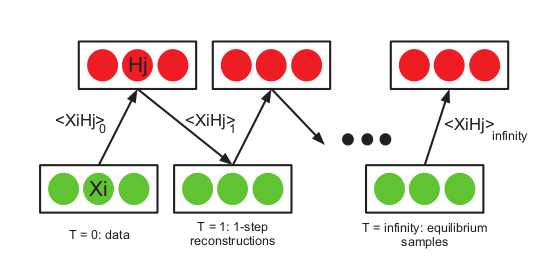
\includegraphics[height=5cm]{rbm_03.png}

Bu yöntem pür Gibbs örneklemesine kıyasla çok daha hızlı işler ve iyi
sonuçlar verir. Teorik olarak niye işlediği [1,2,4] makalelerinde
bulunabilir. CD aslında (4) hedef formülünü değil başka bir hedefi optimize
ediyor, fakat sonuç orijinal gradyan adımlarının yapmak istediğine
yakın. [3] baz alınarak, şu şekilde kodlanabilir,

\inputminted[fontsize=\footnotesize]{python}{rbm.py}

RBM ve Sınıflama 

Sınıflama (classification) işlemi yapmak için BM örneğinde bir
normalizasyon sabiti hesaplamıştık. Burada değişik bir yoldan gideceğiz; ki
bu yol ileride Derin Öğrenim için faydalı olacak. 

Eğittikten sonra bir RBM, içindeki $W$'ye göre, herhangi bir ``görünür''
veri noktası $x$ için bir gizli bir $h$ üretebilir. Bunu üstteki
formülasyondan zaten biliyoruz. Ayrıca, $h$ genellikle daha az boyutta
olduğuna göre (hatta olmasa bile) bu $h$ üretiminin bir tür transformasyon
olduğu, veri üzerinde bir ``özetleme'' yaptığı iddia edilebilir. O zaman
teorik olarak, görünür veri yerine, görünür veriden üretilen gizli veriyi
kullanırsak ve bu veriyi alıp başka bir sınıflayıcıya verirsek, mesela
lojistik regresyon gibi, bu $h$'ler ve etiketler üzerinden denetimli
(supervised) bir eğitim yapabiliriz. Yani, önce RBM eğitiyoruz, tüm verinin
$h$ karşılığını alıyoruz, sonra bunları lojistik regresyona
veriyoruz. Alttaki kodda bunun örneğinin görebiliriz.

Bu kod, ayrıca, k-Katlama (k-fold) tekniğini uyguluyor, veriyi 3 parçaya
bölüp sırasıyla tüm parçaları birer kez test, diğerlerini eğitim verisi
yapıyor, böylece verinin tamamı üzerinden eğitim/test yapmış
olunuyor. Sonuç,

\inputminted[fontsize=\footnotesize]{python}{test_rbmkfold.py}

\begin{minted}[fontsize=\footnotesize]{python}
! python test_rbmkfold.py
\end{minted}

\begin{verbatim}
1.0
\end{verbatim}

Başarı yüzde 100! Altta karşılaştırma için KNN tekniği kullandık,

\inputminted[fontsize=\footnotesize]{python}{test_knnkfold.py}

\begin{minted}[fontsize=\footnotesize]{python}
! python test_knnkfold.py
\end{minted}

\begin{verbatim}
0.98009506833
\end{verbatim}

Kaynaklar

[1] Hinton, G., 
    {\em Training Products of Experts by Minimizing Contrastive Divergence}

[2] Louppe, G., 
    {\em Collaborative filtering, Scalable approaches using restricted Boltzmann machines}, Master Tezi, 2010

[3] \url{https://github.com/echen/restricted-boltzmann-machines}

[4] Tieleman, Hinton, {\em Using Fast Weights to Improve Persistent Contrastive Divergence}

[5] Larochelle, H., {\em Neural networks [5.1] : Restricted Boltzmann machine - definition}, 
    \url{https://www.youtube.com/watch?v=p4Vh_zMw-HQ}

\end{document}
